\Problem{Steady Block on a Sliding Ramp}{\SteadyBlock}{
A block of mass $m$ sits upon a frictionless ramp (inclined at angle $\theta$) that is being pushed to the right. What must the acceleration of the ramp be to prevent the block from sliding down the surface?
}
\ProblemFig{\SteadyBlockFig}{
\centering
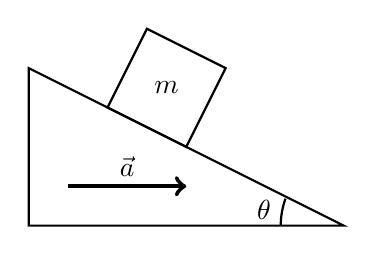
\begin{tikzpicture}
	\draw[thick] (0,0) -- (4,0) -- (0,2) -- cycle;
	\draw[thick] (3.2,0) arc (180:160:1);
	\node[anchor=east] at (3.2,0.2) {$\theta$};
	\draw[thick] (1,1.5) -- (2,1) -- (2.5,2) -- (1.5,2.5) -- cycle;
	\node at (1.75,1.75) {$m$};
	\draw[ultra thick,->] (0.5,0.5) -- (2,0.5);
	\node[anchor=south] at (1.25,0.5) {$\vec{a}$};
	\if\GrayProb1
	\draw (4,1) -- (6,1);
	\node[anchor=west] at (6,1) {$x$};
	\draw (5,0) -- (5,2);
	\node[anchor=south] at (5,2) {$y$};
	\draw[thick] (5,1.5) arc (90:71:0.8);
	\node[anchor=west] at (4.95,1.7) {$\theta$};
	\draw[ultra thick,blue,->] (5,1) -- (5.5,2);
	\node[anchor=west] at (5.5,2) {$\vec{F}^{N}_{BR}$};
	\draw[ultra thick,blue,->] (5,1) -- (5,0);
	\node[anchor=south west] at (5,0) {$\vec{F}^{g}_{BE}$};
	\filldraw[black] (5,1) circle (4pt);
	\draw[ultra thick,red,->] (4.25,1.5) -- (4.75,1.5);
	\node[anchor=south] at (4.5,1.5) {$\vec{F}_{net}$};
	\fi
\end{tikzpicture}
}
\Solution{\SteadyBlockSol}{

If the block is not sliding down the surface of the ramp, then it is moving with it, so the acceleration of the block must be the same as that of the ramp, which points directly to the right. Since we know the direction of acceleration, it will be advantageous to set up our coordinate system with one of the axes along that direction. This differs from several other ramp problems, where a tilted coordinate system is advantageous due to there being fewer vectors to break into components.

If acceleration is along the $x$-axis, as depicted above, we need the two forces (the force on the block normal to the surface of the ramp and the force of gravity on the block) to cancel in the $y$-direction. As such,
\[
0=F^{N}_{BR,y}+F^{g}_{BE,y}=F^{N}_{BR}\cos\theta-mg \implies F^{N}_{BR}\cos\theta=mg \implies F^{N}_{BR}=\frac{mg}{\cos\theta}.
\]
Meanwhile, in the $x$-direction, we only have the $x$-component of the normal force, so
\[
F_{net,x} = F^{N}_{BR,x} = F^{N}_{BR}\sin\theta = mg\frac{\sin\theta}{\cos\theta} = mg\tan\theta.
\]
Since $F_{net,x}=ma_{x}=ma$, we can cancel out the mass to obtain
\[
a = g\tan\theta.
\]
In the special case of a flat ramp, which we expect does not need to move to keep the box from sliding, we have $\theta=0$, and thus $\tan\theta=0$, so our equation indeed gives us $a=0$. Alternatively, if the ramp is vertical, then we cannot keep the block from sliding, as there is nothing beneath it to hold it up. This is the $\theta\to90^{\circ}$ case, and that gives us $a=g\tan\theta\to\infty$, since there is not a finite acceleration sufficient to hold up the block.
}